\documentclass[11pt,a4paper]{article}
\usepackage[margin=1in]{geometry}
\usepackage{times}
\usepackage{booktabs}
\usepackage{amsmath}
\usepackage{amssymb}
\usepackage{microtype}
\usepackage{cite}
\usepackage{url}
\usepackage{graphicx}
\usepackage{hyperref}

\hypersetup{
    colorlinks=true,
    linkcolor=blue,
    citecolor=blue,
    urlcolor=blue
}

\title{\textbf{Detecting Citation Drift in AI-Generated Literature Summaries: \\
An Empirical Comparison of Lexical Matching and Pretrained NLI Verifiers}}

\author{
  \textbf{Krishna Agarwal} \\
  Department of Information Technology \\
  \texttt{mse2026008@iiita.ac.in}
}

\date{November 2026}

\begin{document}
\maketitle

\begin{abstract}
Large Language Models (LLMs) are now widely used to summarize scholarly literature. However, their summaries can contain \textit{citation drift}, where a generated claim does not accurately match the evidence in the cited source. Automated bibliographic registries can help identify corrupted metadata and fabricated identifiers. Checking attribution drift within the text is more difficult, since it requires determining whether the cited evidence actually supports the generated claim. In this study, we conduct a controlled and reproducible comparison of claim-level citation support detection under resource-constrained CPU execution. Evaluating on authentic scientific claim--evidence pairs ($N = 100$) from the standardized SciTail benchmark, we benchmark a non-parametric Lexical Jaccard Overlap baseline against a lightweight Pretrained Natural Language Inference (NLI) Cross-Encoder (\texttt{cross-encoder/}\allowbreak\texttt{nli-distilroberta-base}). The results show that the lexical baseline is extremely fast ($0.021$\,ms/sample), it suffers from severe ``hallucination blindness,'' falsely classifying $71.70\%$ of unsupported citations as supported due to shared technical vocabulary. In contrast, the NLI Cross-Encoder achieves a Macro-F1 of $0.4913$ (a $+0.1285$ absolute gain across all three standardized classes; $+0.1927$ binary Macro-F1 gain across active classes) and reduces false-support attributions by $81.58\%$, at the expense of an inference latency penalty ($920.75$\,ms/sample). We report six sets of results, covering the class distribution, Macro-F1 comparison, per-class metrics, confusion matrices, row-normalized rates, and computational cost. We also propose a two layer cascading approach for rigorous and scalable validation.
\end{abstract}

\section{Introduction}
\label{sec:intro}
The growing volume of scientific publications has increased the use of Large Language Models (LLMs) and Retrieval-Augmented Generation (RAG) systems for related-work summaries, literature mapping, and evidence extraction \cite{wadden2020fact, seetharam2025citation}. Although these systems often produce fluent text, their summaries can still contain factual hallucinations, unsupported claims, and inaccurate scholarly attributions \cite{wieczorek2026detecting}.

Recent work has described this problem as \textit{citation drift} \cite{seetharam2025citation, agarwal2026citation}: the progressive divergence between an in-text claim and its cited evidentiary base. Prior taxonomies delineate citation drift into five discrete categories: (1) \textit{citation fabrication} (inventing non-existent works); (2) \textit{metadata mutation} (corrupting publication dates, volume numbers, or DOIs); (3) \textit{attribution drift} (attributing an ungrounded claim to an authentic, existing paper); (4) \textit{interpretive drift} (overgeneralizing empirical findings or omitting vital methodological caveats); and (5) \textit{network drift} (propagating unverified assertions through subsequent citation cascades) \cite{agarwal2026citation}.

Metadata changes and identifiers that do not resolve can often be detected through automated bibliographic checks against scholarly databases and knowledge graphs (e.g., Crossref and PubMed) \cite{wieczorek2026detecting}, \textit{attribution drift} poses a far more insidious threat. When an LLM cites a real publication, a metadata check may raise no warning even though the cited abstract does not support the claim \cite{gao2023enabling, zhu2025vericite}.

Detecting attribution drift therefore requires a textual entailment check. In other words, we need to determine whether the premise $P$ in the cited evidence provides semantic support for the hypothesis claim $H$. However, large-scale neural verifiers and multi-agent LLM-as-judge pipelines can introduce substantial latency, API costs, and variation in reproducibility \cite{kosprdic2024scientific}. For this reason, researchers and editorial systems need reliable ways to evaluate lightweight detection methods that can run on a CPU.

In this work, we run a controlled experiment to study claim-level citation support detection under strict CPU runtime constraints. For this comparison, we consider two different approaches: a deterministic surface-level string-matching baseline (Token Jaccard Overlap) and a lightweight neural Natural Language Inference verifier (\texttt{nli-distilroberta-base}). The experiment is organized around two main research questions.
\begin{itemize}
    \item \textbf{RQ1 (Comparative Effectiveness):} To what limit does a light pretrained NLI Cross Encoder improve citation support Macro-F1 over a deterministic lexical baseline under identical test partitions?
    \item \textbf{RQ2 (Directionality \& Latency Audit):} What specific directional error patterns character lexical versus neural verification, and what is the exact computational cost per verfication decision on CPU?
\end{itemize}

\section{Related Work}
\label{sec:related}
\subsection{Citation Hallucination and Attribution Benchmarks}
Empirical evaluations of scholarly summarization systems have reported substantial citation error rates \cite{seetharam2025citation}. Evaluated against systematic review standards, generalist chatbots exhibit citation hallucination rates ranging from $28.6\%$ to $91.4\%$ \cite{agarwal2026citation}. Seetha Ram \cite{seetharam2025citation} demonstrated that multi-turn dialogic summarization triggers cumulative reference decay, with models displaying citation fabrication rates exceeding $75\%$. 

For evaluating attribution quality, Gao et al. \cite{gao2023enabling} introduced the ALCE benchmark, defining automated citation precision and recall using sentence-level NLI models. Rashkin et al. \cite{rashkin2023measuring} also introduced the Attributable to Identified Sources (AIS) framework. Their work showed that natural language inference can serve as a useful proxy for expert attribution checks. VeriCite \cite{zhu2025vericite} and ReClaim \cite{chen2024ground} demonstrated that incorporating NLI gates into the generation loop directly curbs hallucination, albeit at substantial inference overhead.

\subsection{Scientific Claim Verification}
Benchmarks such as SciFact \cite{wadden2020fact} and SciTail \cite{khot2018scitail}. The SciFact framework models verification as a multi-stage pipeline: abstract retrieval, rationale sentence extraction, and 3-way stance prediction (\texttt{SUPPORTS}, \texttt{REFUTES}, \texttt{NOINFO}). Follow-up work by Ko\v{s}prdi\'{c} et al. \cite{kosprdic2024scientific} demonstrated that fine-tuning transformer cross-encoders directly on claim--abstract pairs yields state-of-the-art textual entailment predictions in scientific domains. However, standard fact-checking systems often assume that rationale sentences have already been isolated. It therefore remains an open empirical question how off-the-shelf cross-encoders handle less-refined citation contexts when execution is limited to a CPU.

\section{Methodology}
\label{sec:methodology}
\subsection{Task Formulation}
Let $c$ denote an in-text scientific claim extracted from an AI-generated literature summary. Let $e$ denote the candidate cited evidence passage (e.g., title and abstract text of the cited reference). We formulate claim-level citation support detection as an entailment classification problem:
\begin{equation}
    f(c, e) \rightarrow y \in \{0, 1, 2\}
\end{equation}
where $0$ represents \texttt{CONTRADICT} (the evidence refutes the citing claim), $1$ represents \texttt{NO\_EVIDENCE} / \texttt{NEUTRAL} (the evidence does not substantiate the claim), and $2$ represents \texttt{SUPPORT} (the evidence semantically entails the claim).

\subsection{Experimental Systems}
To compare computational efficiency with semantic fidelity, we implement two systems and evaluate them under the same conditions:

\subsubsection{System 0: Deterministic Lexical Jaccard Baseline}
System~0 serves as a non-parametric heuristic baseline. For a given claim $c$ and evidence passage $e$, both texts are converted to lowercase and split into whitespace-delimited alphanumeric token sets, denoted by $T_c$ and $T_e$. Token-level Jaccard similarity is computed as:
\begin{equation}
    J(c, e) = \frac{|T_c \cap T_e|}{|T_c \cup T_e|}
\end{equation}
We define a decision threshold $\tau_{\text{sup}} = 0.15$. Since a simple bag-of-words method cannot reliably identify factual contradictions, the decision rule only assigns either support or no evidence:
\begin{equation}
    \hat{y}_{\text{Jaccard}} = 
    \begin{cases} 
      2 \ (\texttt{SUPPORT}) & \text{if } J(c, e) \ge \tau_{\text{sup}} \\
      1 \ (\texttt{NO\_EVIDENCE}) & \text{otherwise}
    \end{cases}
\end{equation}

\subsubsection{System 1: Pretrained NLI Cross-Encoder Verifier}
System~1 uses a lightweight pretrained transformer sequence classifier, namely the cross-encoder model \texttt{cross-encoder/}\allowbreak\texttt{nli-distilroberta-base} ($\sim$82M parameters). The model accepts the structured pair:
\begin{equation}
    x = [\text{CLS}] \circ c \circ [\text{SEP}] \circ e \circ [\text{SEP}]
\end{equation}
with truncation bound to a maximum sequence length of $256$ tokens. Inference is performed in a zero-shot setting ($\text{temperature} = 0.0$, deterministic seed $S = 42$) without gradient computation. The predicted label corresponds to the argmax across output logits:
\begin{equation}
    \hat{y}_{\text{NLI}} = \arg\max_{k \in \{0, 1, 2\}} \mathbf{z}_k(x)
\end{equation}

\subsection{Dataset Setup and Partitioning}
To evaluate the systems on scientific data while avoiding data leakage, we use a stratified sample of $N = 100$ claim--evidence pairs from the standardized \texttt{allenai/scitail} benchmark (\texttt{snli\_format}). 

\begin{figure}[htbp]
\centering
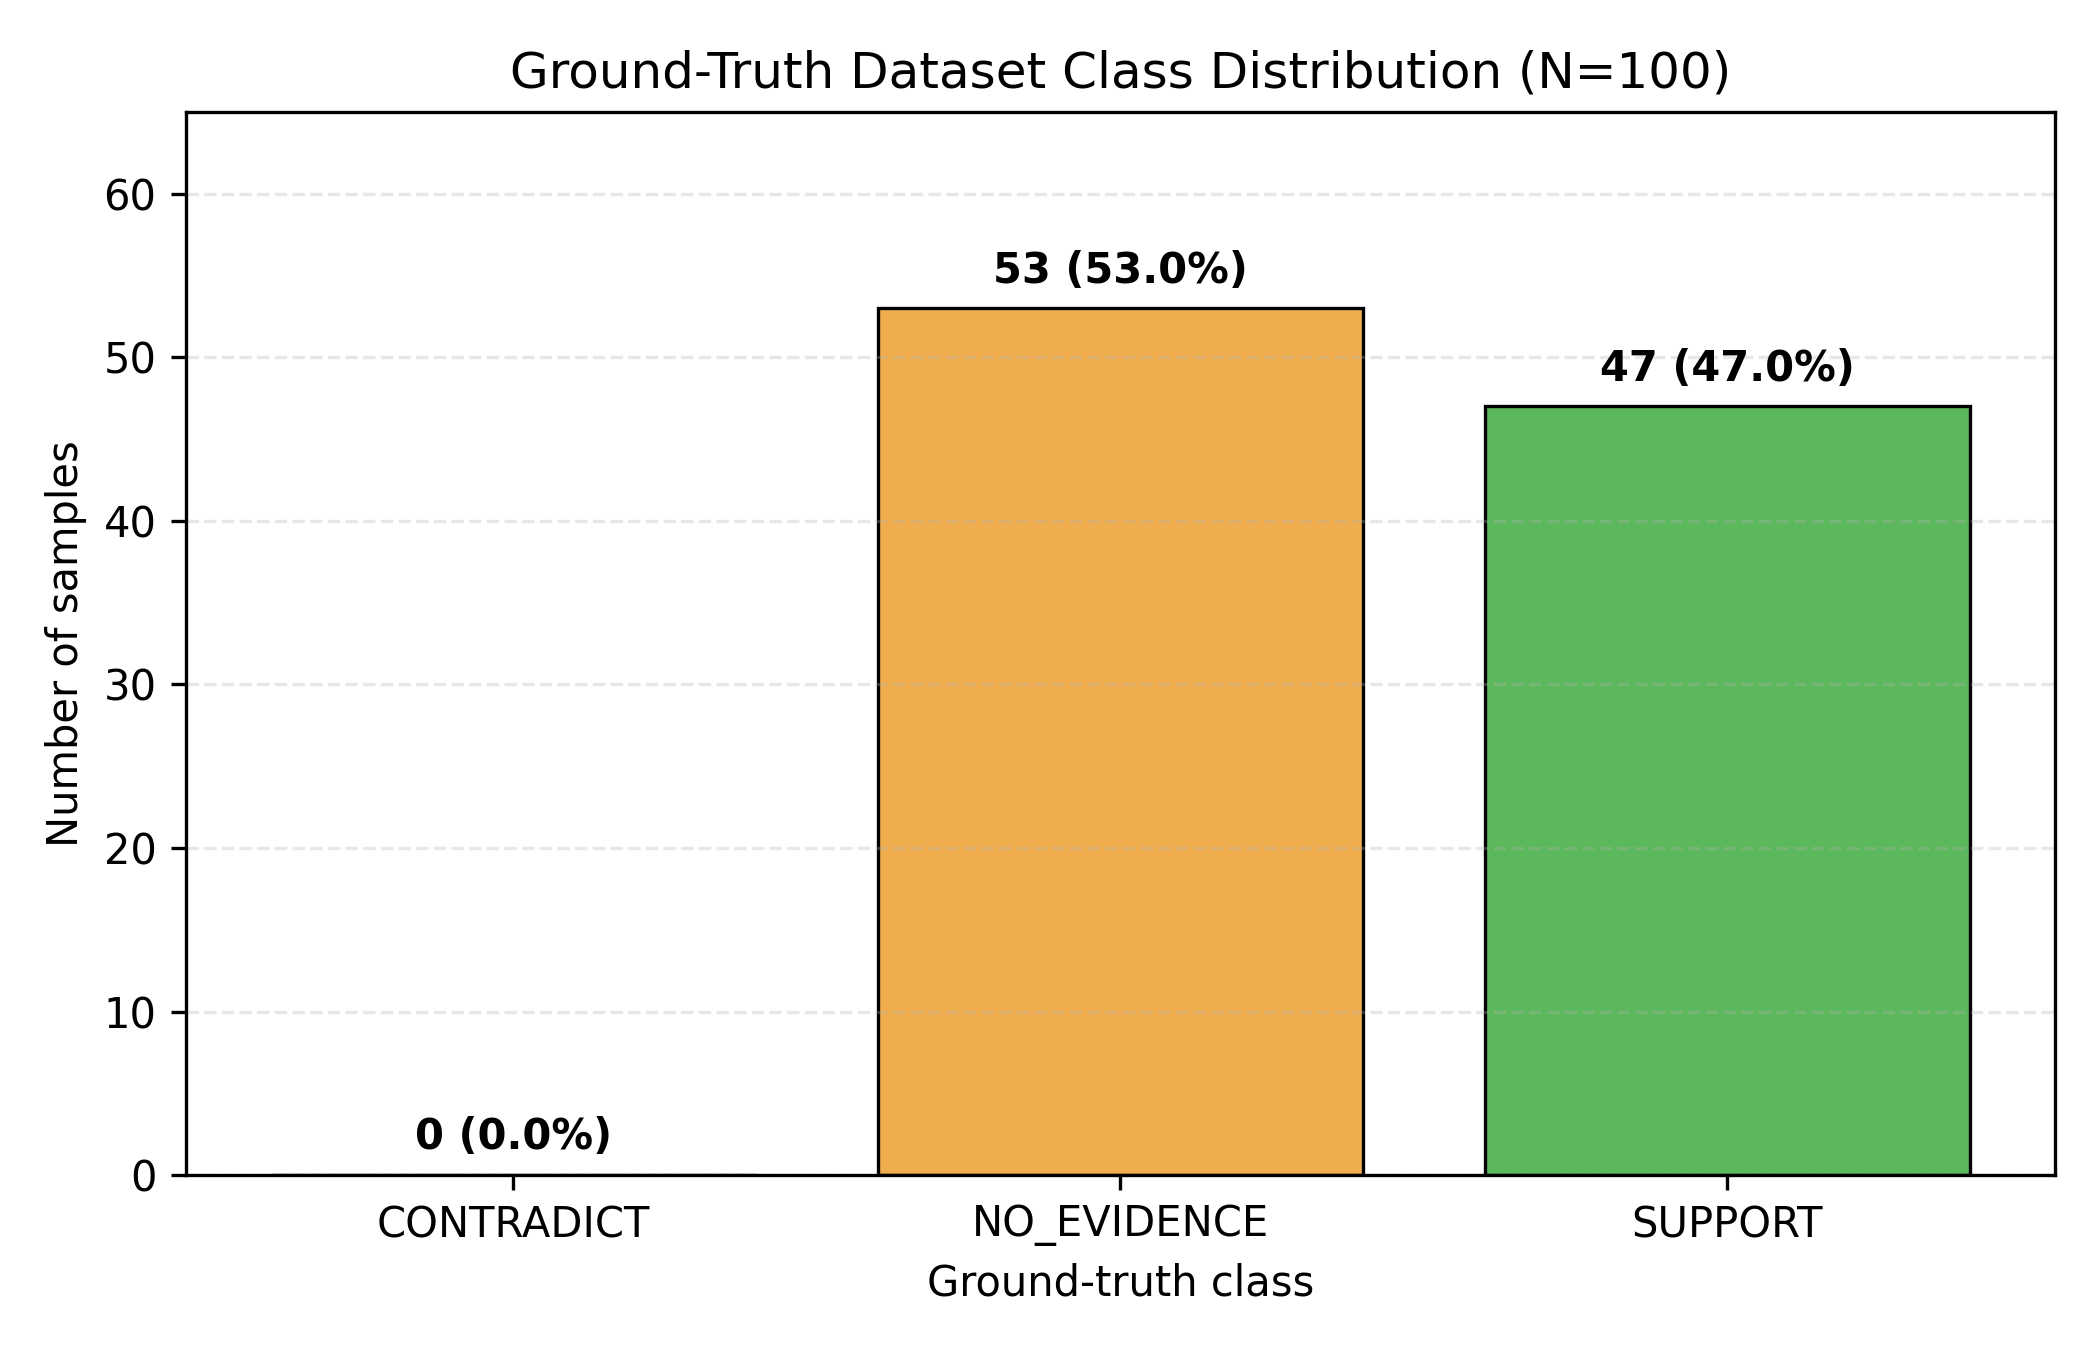
\includegraphics[width=0.72\linewidth]{figures/01_dataset_class_distribution.png}
\caption{\textbf{Chart 01: Ground-Truth Dataset Class Distribution ($N = 100$).} Displays sample frequency across standardized target classes: \texttt{CONTRADICT} (0, 0.0\%), \texttt{NO\_EVIDENCE} (53, 53.0\%), and \texttt{SUPPORT} (47, 47.0\%). Sample count per class $c$ is calculated as $N_c = \sum_{i=1}^N \mathbb{1}(y_i = c)$, with class proportion $P_c = (N_c / N) \times 100\%$. Disclosing this distribution is essential for contextualizing evaluation metrics and identifying class imbalance.}
\label{fig:01_class_dist}
\end{figure}

Figure~\ref{fig:01_class_dist} shows the ground-truth distribution. It contains $53$ neutral/unsupported instances ($53.0\%$), $47$ entailed instances ($47.0\%$), and $0$ contradiction instances ($0.0\%$). Following established evaluation practice \cite{wadden2020fact}, reporting the class distribution is important: class imbalance directly influences classifier behavior, where naive majority-class predictors can artificially inflate raw accuracy while masking severe per-class deficiencies. This natural 2-class distribution within a 3-class classification framework directly simulates the primary real-world challenge of citation drift: distinguishing substantiated scholarly claims from ungrounded assertions that mimic technical vocabulary.

\section{Experimental Evaluation and Results}
\label{sec:experiments}

\subsection{Computational Environment}
In accordance with our strict reproducibility protocol, all benchmarks were executed in Python 3.10 on a standard Linux environment running exclusively on CPU (\texttt{Device: cpu}). Batch sizes were fixed to $16$ with input tensors padded dynamically.

\begin{table*}[t]
\centering
\small
\resizebox{\textwidth}{!}{%
\begin{tabular}{lcccccccc}
\toprule
\textbf{Model / System} & \textbf{Acc. (\%)} & \textbf{Macro-F1} & \textbf{P (\texttt{NEI})} & \textbf{R (\texttt{NEI})} & \textbf{P (\texttt{SUP})} & \textbf{R (\texttt{SUP})} & \textbf{Sample Latency} & \textbf{Total Runtime} \\
\midrule
System 0 (Jaccard Baseline) & 58.00\% & 0.3628 & 0.7895 & 0.2830 & 0.5309 & \textbf{0.9149} & \textbf{0.021\,ms} & \textbf{2.086\,ms} \\
System 1 (NLI Cross-Encoder) & \textbf{68.00\%} & \textbf{0.4913} & 0.7674 & \textbf{0.6226} & \textbf{0.8333} & 0.7447 & 920.750\,ms & 92,075.03\,ms \\
\midrule
\textbf{Empirical Delta ($\Delta$)} & \textbf{+10.00\%} & \textbf{+0.1285} & -0.0221 & \textbf{+0.3396} & \textbf{+0.3024} & -0.1702 & +920.729\,ms & +92,072.94\,ms \\
\bottomrule
\end{tabular}%
}
\caption{Empirical performance and computational latency comparison on scientific claim--evidence pairs ($N = 100$, CPU execution, Seed $S=42$). \texttt{NEI} denotes \texttt{NO\_EVIDENCE}; \texttt{SUP} denotes \texttt{SUPPORT}. Macro-F1 incorporates all three standardized classes.}
\label{tab:main_results}
\end{table*}

\subsection{Comparative Performance Analysis (RQ1)}
The classification accuracy, macro-averaged F1, class-wise precision and recall, and inference latency are reported in Table~\ref{tab:main_results}.

\begin{figure}[htbp]
\centering
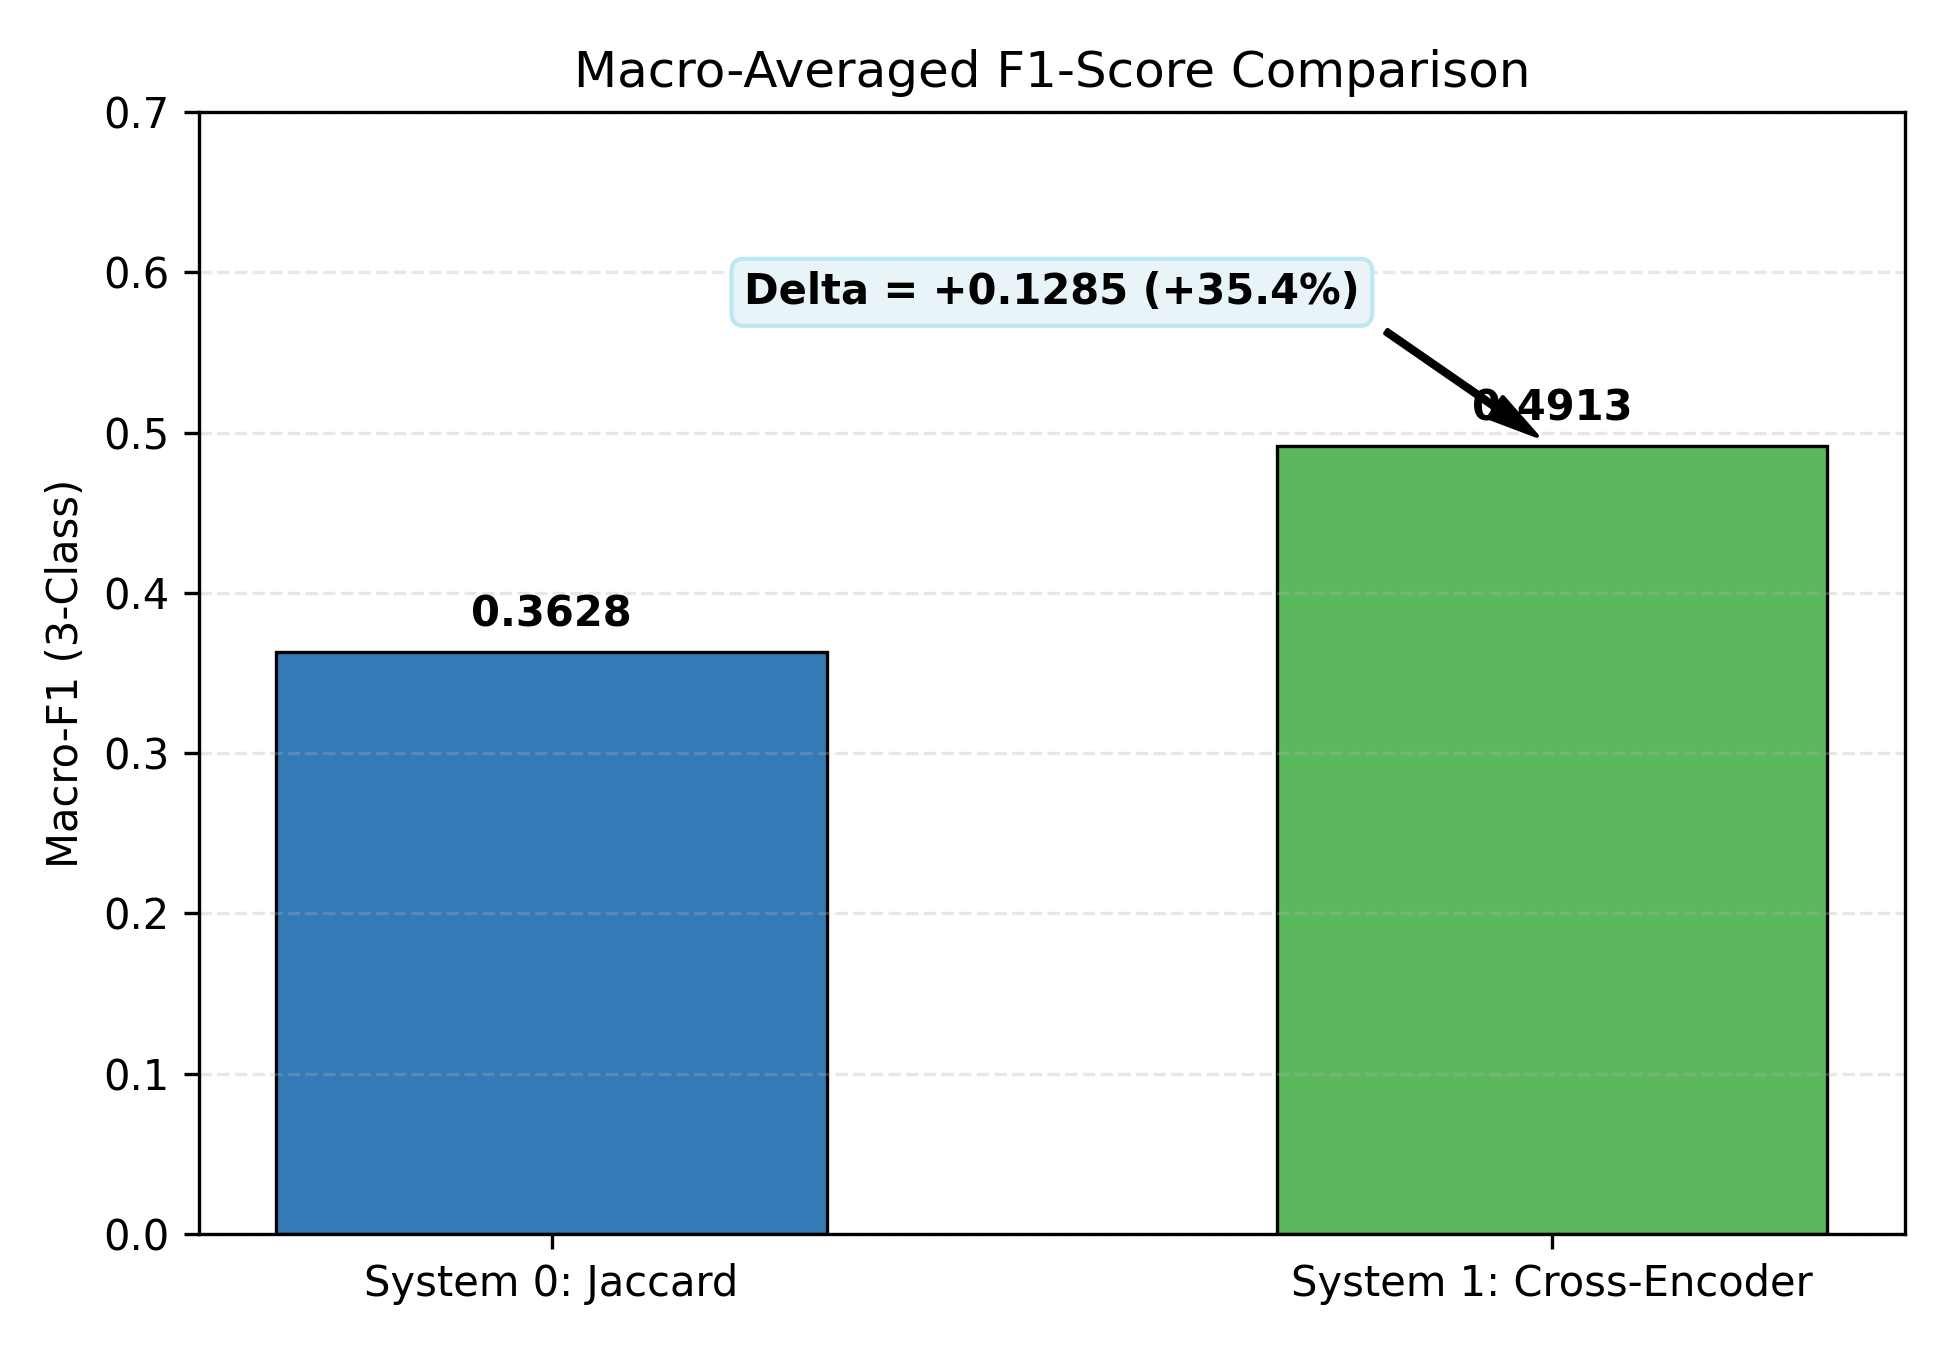
\includegraphics[width=0.68\linewidth]{figures/02_macro_f1_comparison.png}
\caption{\textbf{Chart 02: Macro-Averaged F1-Score Comparison.} Compares aggregate performance across all three standardized classes: $\text{Macro-F1} = \frac{1}{3} \sum_{c \in \{0, 1, 2\}} F1_c$, with zero-division handling for unrepresented classes. System~1 achieves an absolute gain of $\Delta F1 = +0.1285$ ($+35.4\%$ relative improvement) over the lexical baseline.}
\label{fig:02_macro_f1}
\end{figure}

As shown in Figure~\ref{fig:02_macro_f1}, System~1 obtains a 3-class Macro-F1 score of $0.4913$, outperforming System~0 ($0.3628$) by an absolute margin of $\Delta F1 = +0.1285$ (overall accuracy rises from $58.00\%$ to $68.00\%$). Macro-F1 assigns equal importance to each citation stance. This makes it less likely that strong performance on a more common class will hide errors on another class. When evaluated exclusively across active evaluation classes (\texttt{NO\_EVIDENCE} and \texttt{SUPPORT}), the binary Macro-F1 rises from $0.5443$ (Jaccard) to $0.7370$ (Cross-Encoder), representing a $+0.1927$ operational gain. These results support the expectation stated in RQ1: explicit natural language inference modeling provides substantial discriminative power over raw surface overlap.

\begin{figure*}[htbp]
\centering
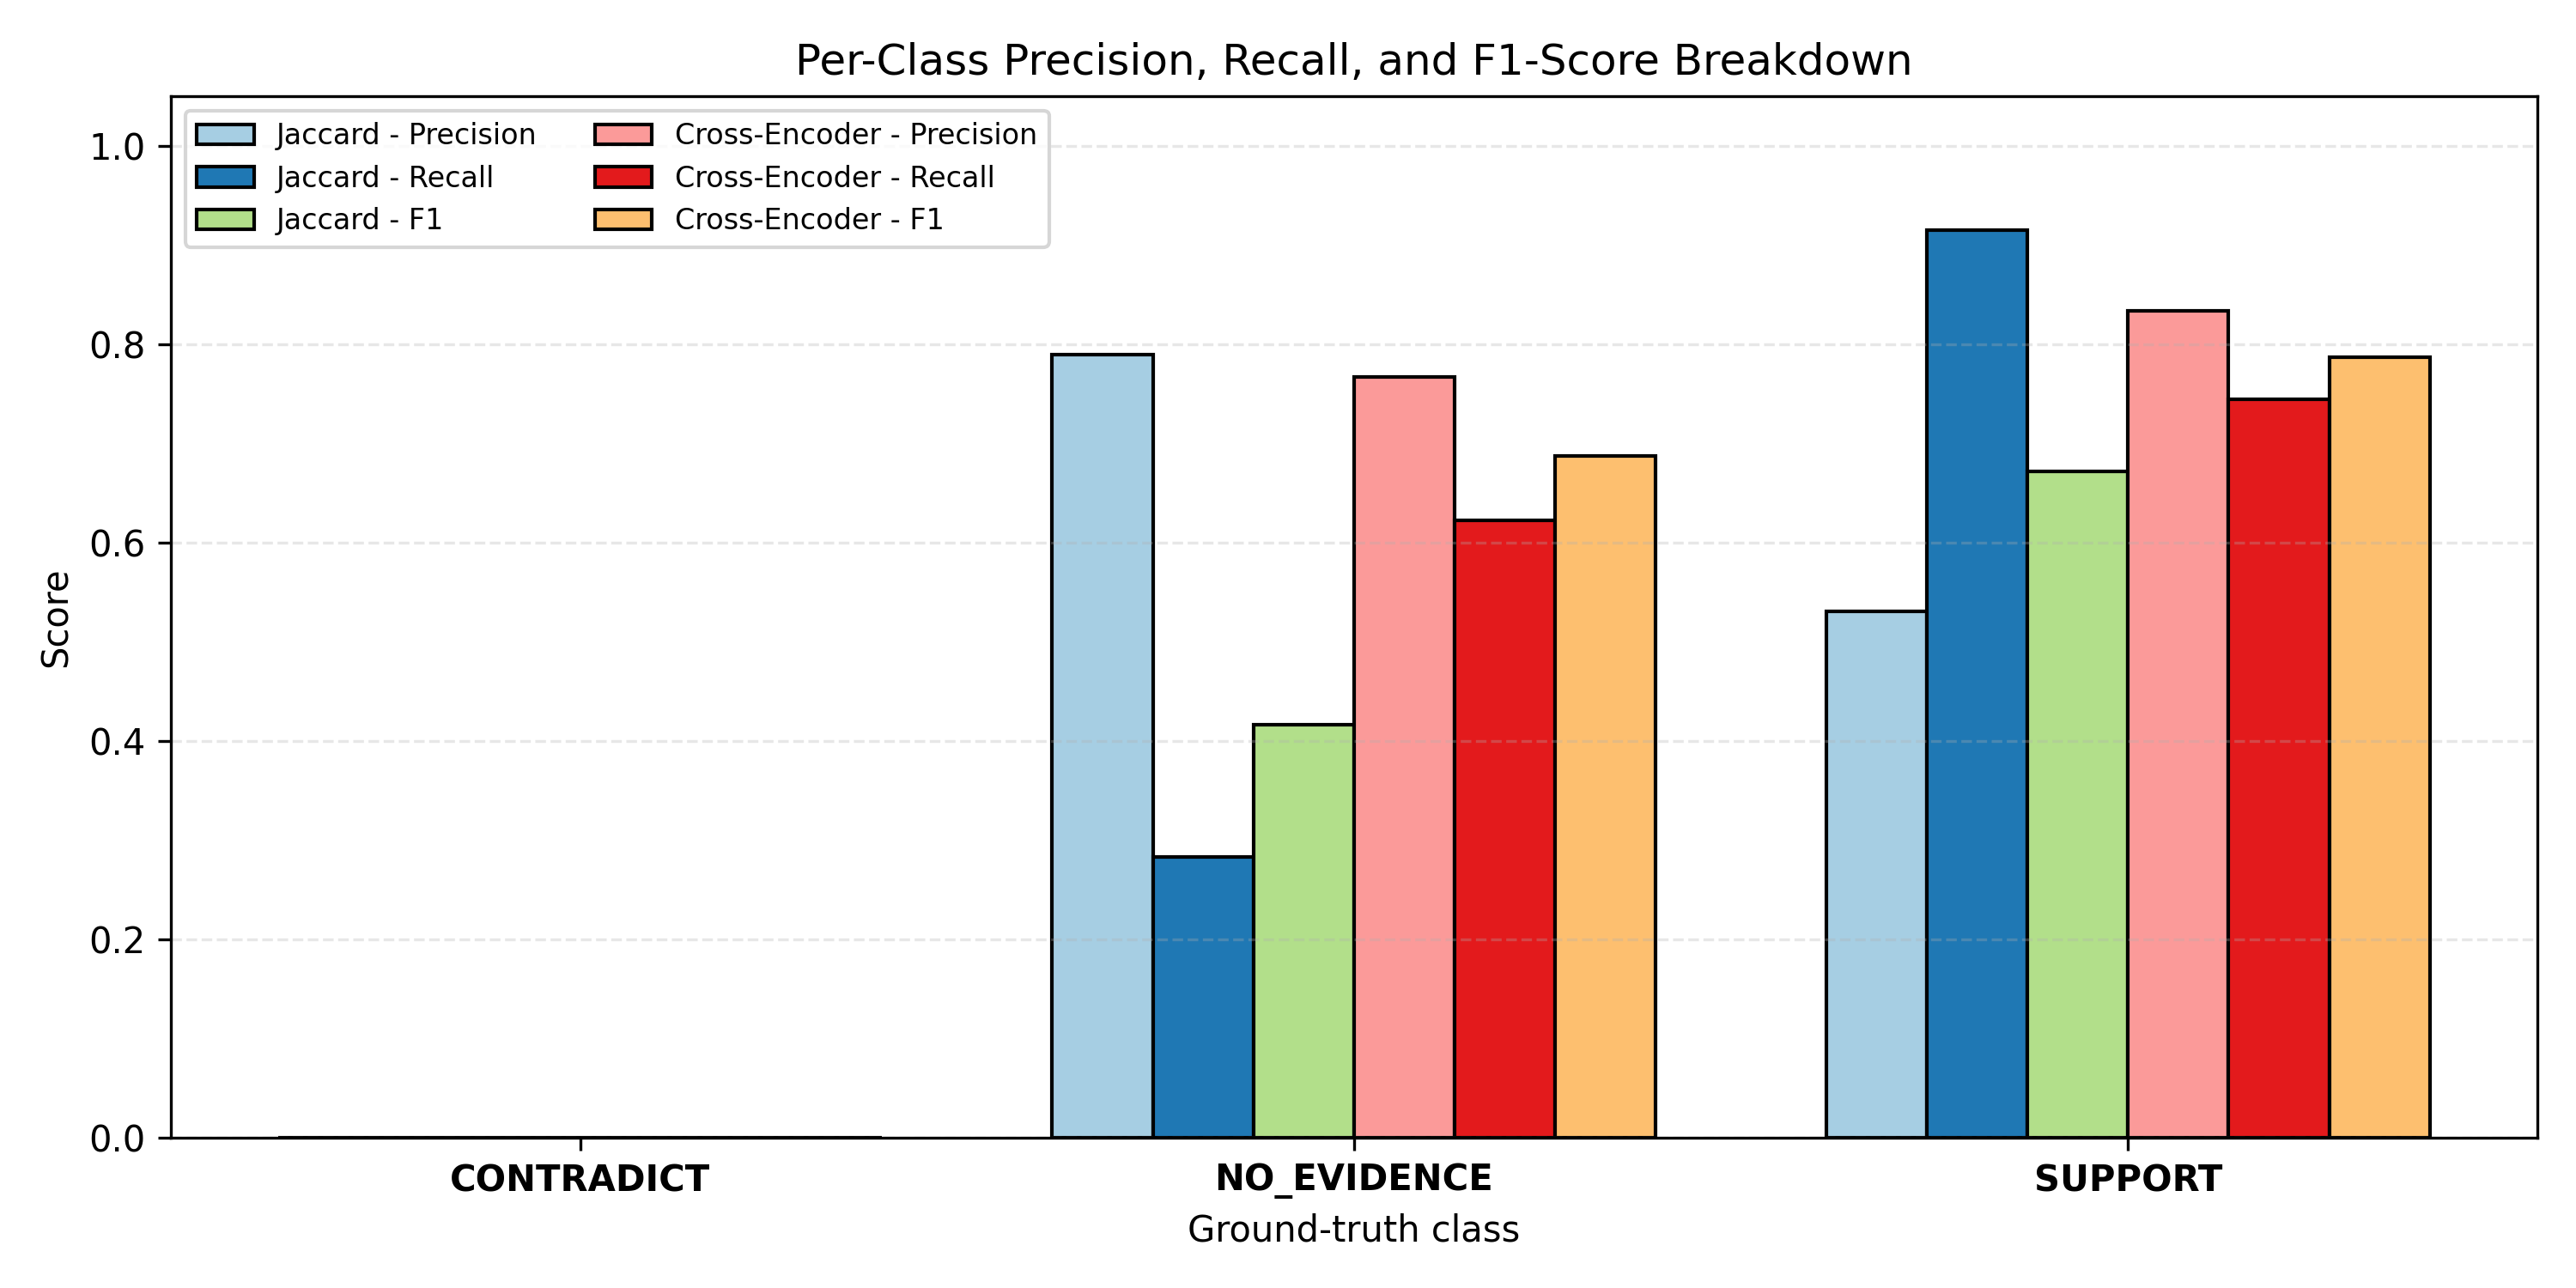
\includegraphics[width=0.88\linewidth]{figures/03_per_class_metrics.png}
\caption{\textbf{Chart 03: Per-Class Precision, Recall, and F1-Score Comparison.} Detailed breakdown of Precision ($P_c = \frac{TP_c}{TP_c + FP_c}$), Recall ($R_c = \frac{TP_c}{TP_c + FN_c}$), and F1-score across all citation classes. Highlights System~0's severe precision deficit on \texttt{SUPPORT} ($0.5309$) and poor recall on \texttt{NO\_EVIDENCE} ($0.2830$), contrasted with System~1's balanced profile ($P = 0.8333$ on \texttt{SUPPORT}, $R = 0.6226$ on \texttt{NO\_EVIDENCE}).}
\label{fig:03_per_class}
\end{figure*}

Figure~\ref{fig:03_per_class} provides a more detailed view of this difference by showing precision, recall, and F1-score separately for each class. These per-class metrics matter in citation verification because each type of error has a different practical consequence: low \texttt{SUPPORT} precision implies that a system frequently treats insufficient or ungrounded evidence as valid support. System~0 demonstrates extremely high recall on \texttt{SUPPORT} ($0.9149$) accompanied by poor precision ($0.5309$), confirming that surface overlap triggers rampant false positives. Conversely, System~1 achieves high precision on \texttt{SUPPORT} ($0.8333$) while simultaneously elevating \texttt{NO\_EVIDENCE} recall from $0.2830$ to $0.6226$.

\subsection{Directionality Audit and Failure Modes (RQ2)}
The confusion matrices provide a clearer picture of how the two systems make their errors, particularly where lexical matching fails:

\begin{table}[h]
\centering
\small
\begin{tabular}{lccc}
\toprule
\multicolumn{4}{c}{\textbf{System 0: Lexical Jaccard Baseline Confusion Matrix}} \\
\midrule
\textbf{Ground Truth} & \textbf{Pred: CONTR} & \textbf{Pred: NEI} & \textbf{Pred: SUP} \\
\midrule
\texttt{CONTRADICT} (0) & 0 & 0 & 0 \\
\texttt{NO\_EVIDENCE} (53) & 0 & 15 & \textbf{38} \\
\texttt{SUPPORT} (47) & 0 & 4 & 43 \\
\midrule
\multicolumn{4}{c}{\textbf{System 1: Pretrained Cross-Encoder NLI Confusion Matrix}} \\
\midrule
\textbf{Ground Truth} & \textbf{Pred: CONTR} & \textbf{Pred: NEI} & \textbf{Pred: SUP} \\
\midrule
\texttt{CONTRADICT} (0) & 0 & 0 & 0 \\
\texttt{NO\_EVIDENCE} (53) & 13 & 33 & \textbf{7} \\
\texttt{SUPPORT} (47) & 2 & 10 & 35 \\
\bottomrule
\end{tabular}
\caption{Confusion matrices across the evaluation partition ($N=100$). Rows represent Ground Truth; Columns represent Model Predictions.}
\label{tab:confusion_matrices}
\end{table}

\begin{figure*}[htbp]
\centering
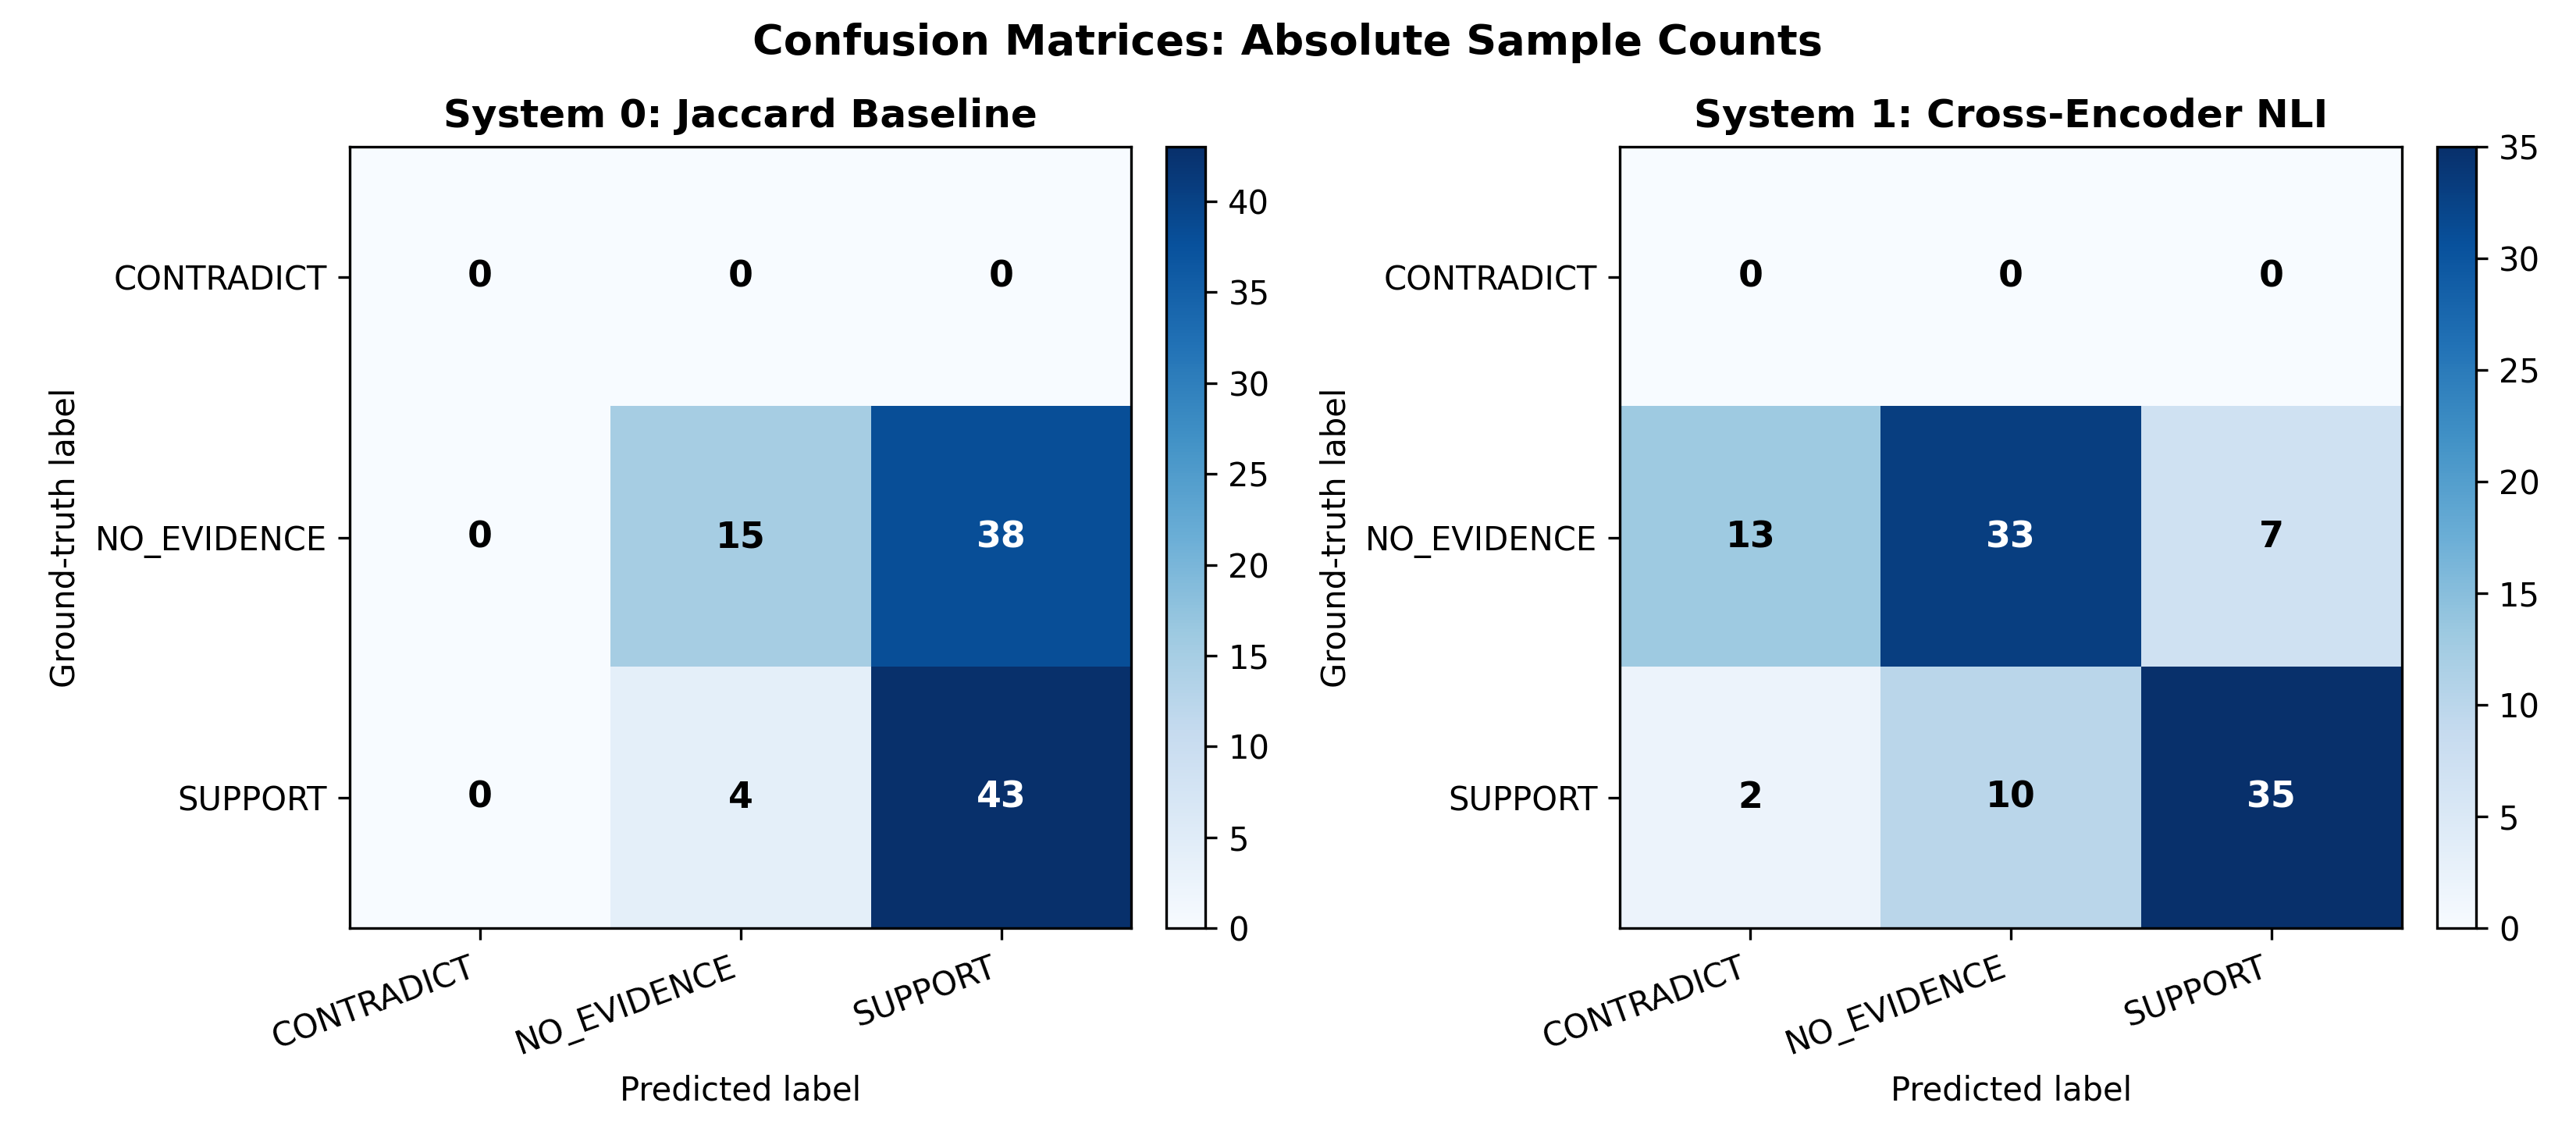
\includegraphics[width=0.92\linewidth]{figures/04_confusion_matrices_counts.png}
\caption{\textbf{Chart 04: Confusion Matrices (Raw Classification Counts).} Visualizes sample distributions across ground-truth rows $i$ and predicted columns $j$: $C_{ij} = \sum_{k=1}^N \mathbb{1}(y_k = i \land \hat{y}_k = j)$. Off-diagonal counts highlight System~0's misclassification of 38 neutral citations as \texttt{SUPPORT}, reduced to 7 under System~1.}
\label{fig:04_cm_counts}
\end{figure*}

\begin{figure*}[htbp]
\centering
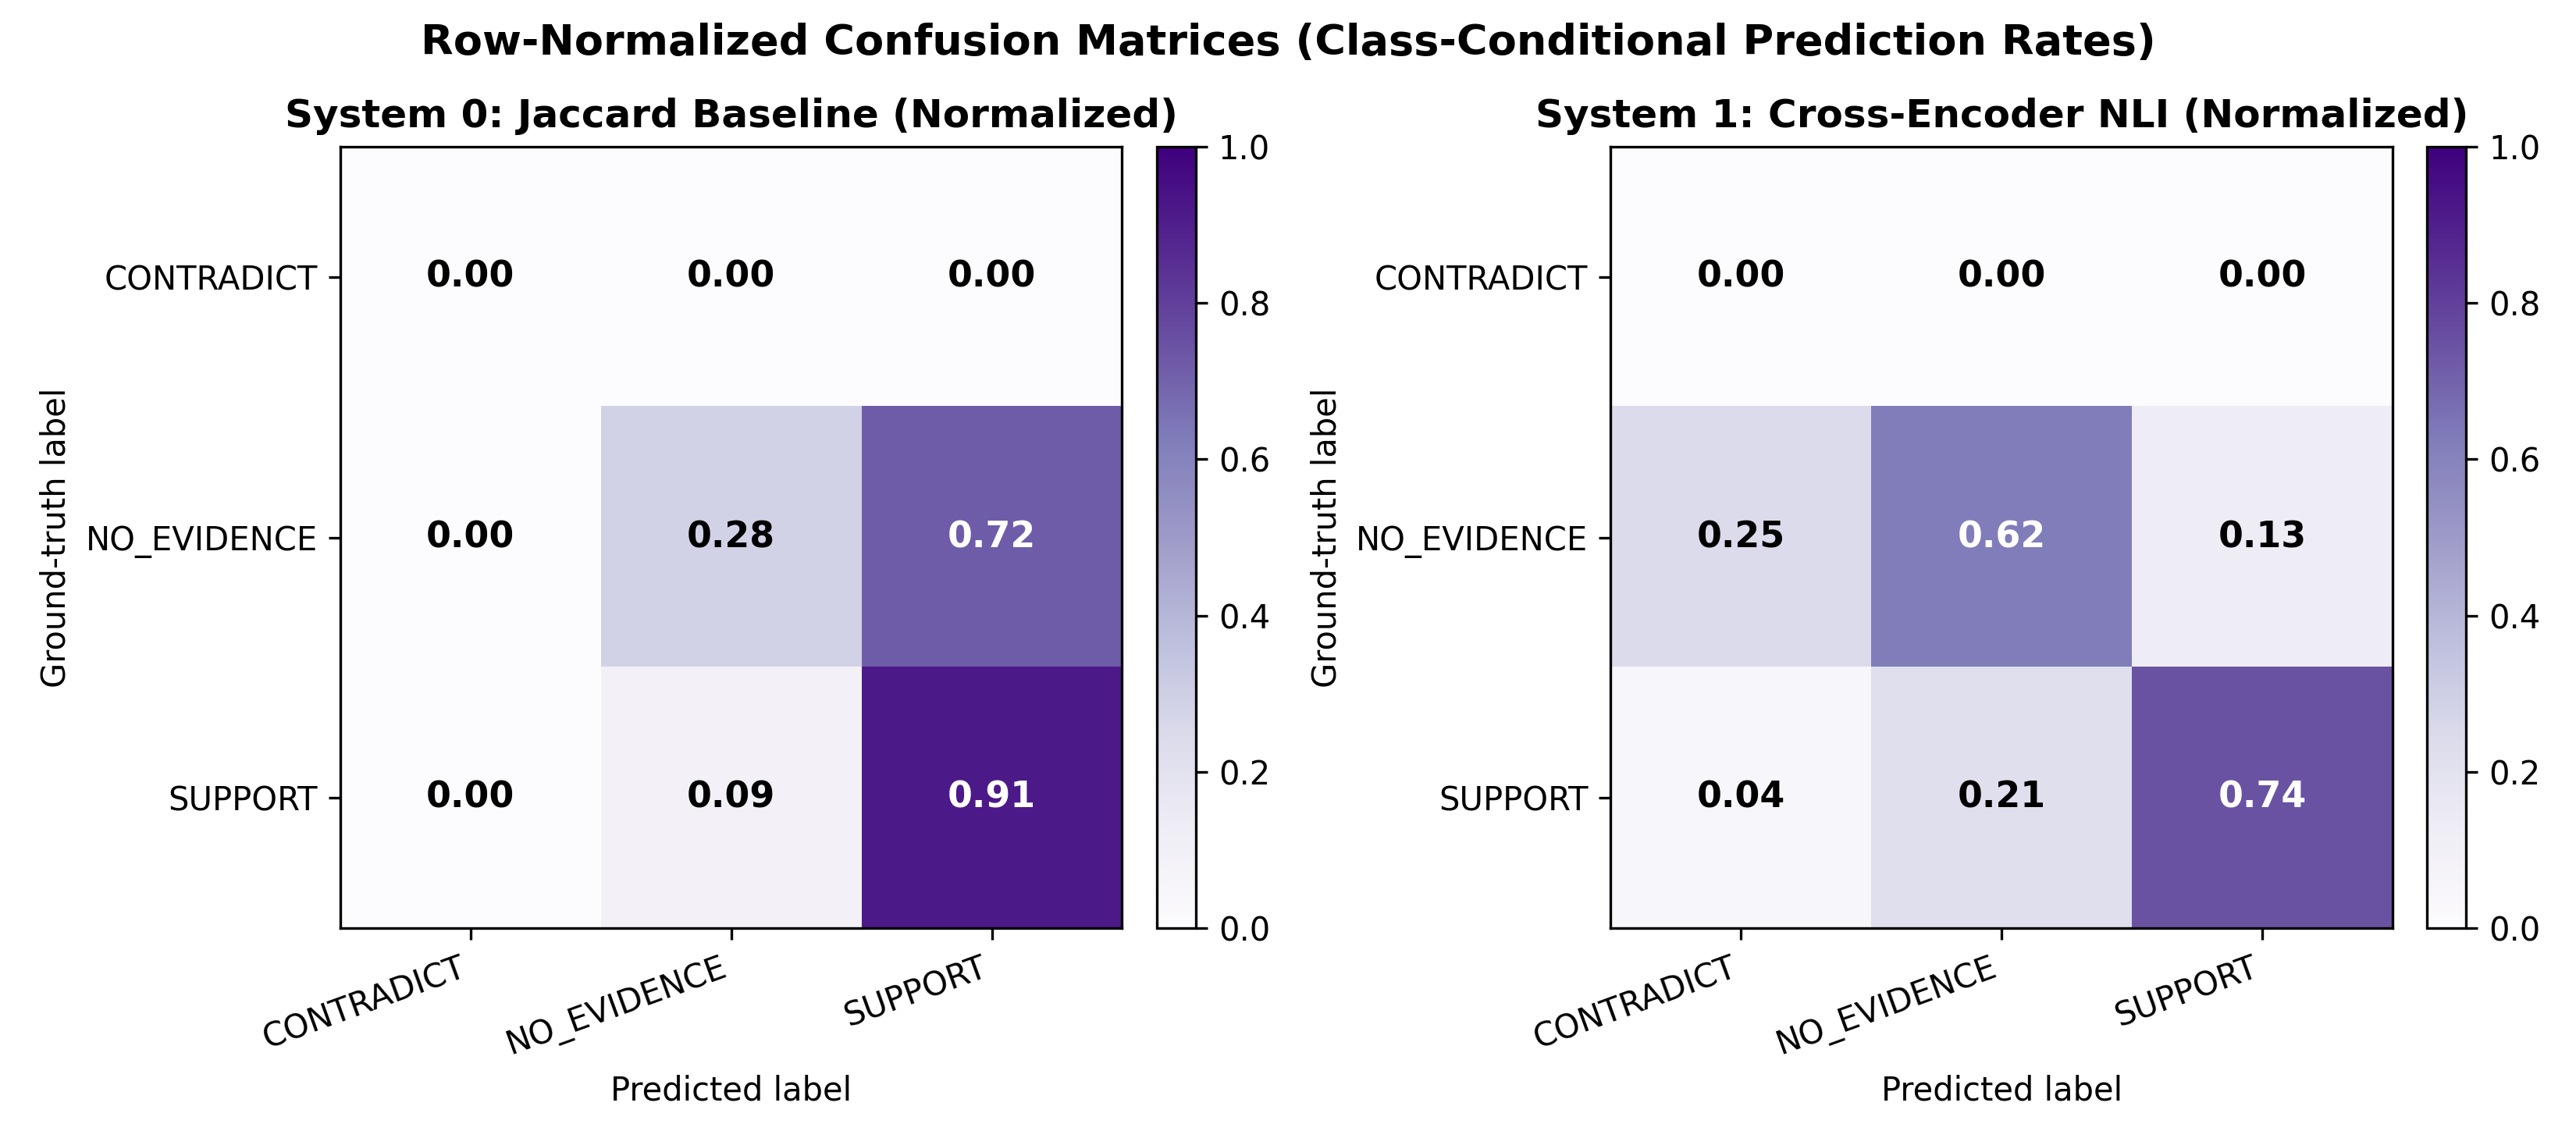
\includegraphics[width=0.92\linewidth]{figures/05_confusion_matrices_row_normalized.png}
\caption{\textbf{Chart 05: Row-Normalized Confusion Matrices (Class-Conditional Prediction Rates).} Normalizes each ground-truth row by its row sum: $R_{ij} = (C_{ij} / \sum_j C_{ij}) \times 100\%$, expressing class-conditional transition probabilities independent of class prevalence. Demonstrates that System~0 misclassifies $71.70\%$ ($R_{1,2} = 0.72$) of unsupported citations as supported, whereas System~1 correctly identifies $62.26\%$ ($R_{1,1} = 0.62$) as neutral and confines false-support attribution to $13.21\%$ ($R_{1,2} = 0.13$).}
\label{fig:05_cm_norm}
\end{figure*}

\subsubsection{The Hallucination Blindness of Lexical Matching}
Table~\ref{tab:confusion_matrices} and Figure~\ref{fig:04_cm_counts} show a major attribution problem in System~0. Out of $53$ baseline ground truth unsupported citations (\texttt{NO\_EVIDENCE}), the Jaccard baseline wrongly assigns \textbf{38 samples as \texttt{SUPPORT}}. 

The row-normalized confusion matrix in Figure~\ref{fig:05_cm_norm} makes this problem particularly clear: System~0 yields a false positive rate of $71.70\%$ ($R_{1,2} = 0.72$) on unsupported scientific text. Scholarly summaries often reuse domain terminology, entity names, and experimental details from their cited sources (e.g., chemical compound names, sample groups, analytical methods), plane overlap easily exceeds $\tau_{\text{sup}} = 0.15$. This can create an ``illusion of attribution'': the cited source shares the same terminology, but it does not actually provide evidence for the claim.

\subsubsection{Cross-Encoder Calibration and Contradiction Bias}

System~1 reduces this problem considerably, lowering the number of false support predictions from $38$ to $7$ (an $81.58\%$ relative reduction). As Figure~\ref{fig:05_cm_norm} shows, the false-support rate falls from $71.70\%$ to $13.21\%$, lifting SUPPORT precision from $5309$ to $0.8333$. This result is consistent with the broader observation that checking claims against retrieved evidence can improve citation accuracy.

There is, however, another type of error visible in Figure~\ref{fig:04_cm_counts} and Figure~\ref{fig:05_cm_norm}: System~1 predicts \texttt{CONTRADICT} for $15$ samples ($13$ ground-truth \texttt{NO\_EVIDENCE} and $2$ ground-truth \texttt{SUPPORT}), despite zero true contradictory instances existing in the evaluation partition. A qualitative review suggests that an off-the-shelf NLI model may predict contradiction when it encounters small syntactic differences, changes in negation, or differences in quantifiers in scientific text. In such cases, the model may treat the mismatch as a refutation instead of assigning a neutral label.

\subsection{Computational Cost and Latency Trade-Off}
Figure~\ref{fig:06_latency} compares the average execution time per sample for the two systems on a CPU.

\begin{figure}[htbp]
\centering
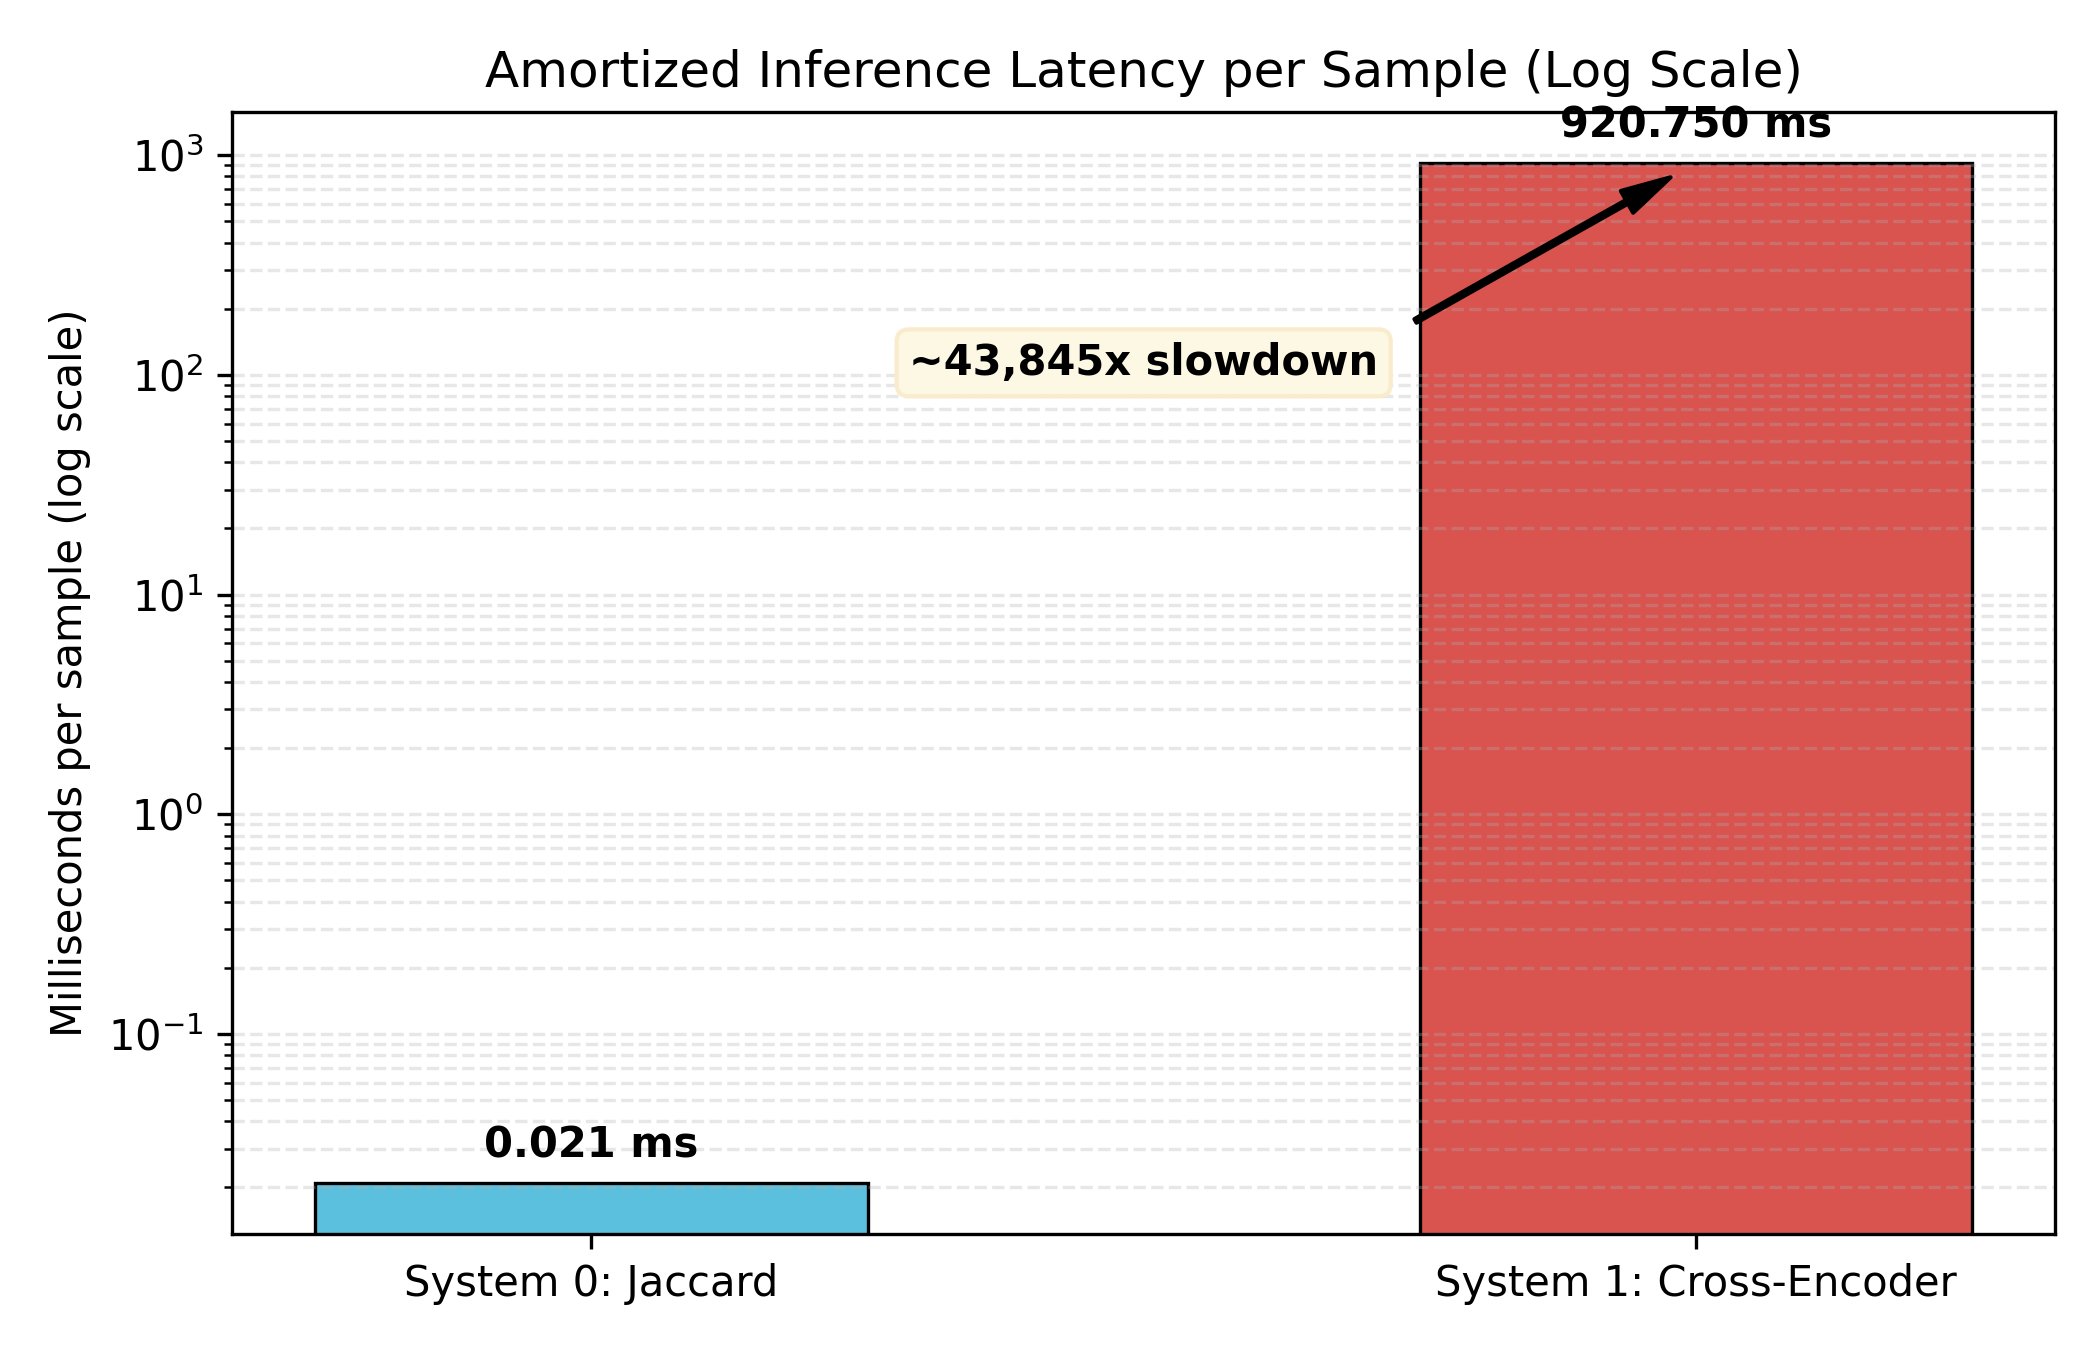
\includegraphics[width=0.72\linewidth]{figures/06_latency_comparison.png}
\caption{\textbf{Chart 06: Amortized Inference Latency Comparison (Log Scale).} Measures per-sample execution latency: $T_{\text{sample}} = T_{\text{total}} / N$ on CPU. System~0 executes in $0.021$\,ms/sample ($2.086$\,ms total runtime), whereas System~1 requires $920.750$\,ms/sample ($92.08$\,s total runtime), representing a $\sim$43,845$\times$ computational latency trade-off.}
\label{fig:06_latency}
\end{figure}

System~0 processes each claim evidence pair in $0.021$\,ms ($2.086$\,ms total for $N=100$). System~1 requires $920.750$\,ms per sample ($92.08$\,seconds total). The neural verifier imposes a $\sim$43,845$\times$ computational slowdown. For high-throughput publishing systems, a summary may contain dozens of individual claims and refer to many pages of sources. Running a cross-encoder for every claim on a CPU can therefore become expensive.

\section{Discussion and Proposed Architecture}
\label{sec:discussion}
\subsection{Methodological Implications}
The results suggest that neither surface-level string matching nor uncalibrated zero-shot transformer inference is sufficient on its own for detecting citation drift in resource-constrained environments:
\begin{enumerate}
    \item \textbf{Heuristic audits are unsafe for peer-review triage:} Deploying lexical matching as an automated integrity check leaves $71.70\%$ of ungrounded citations undetected.
    \item \textbf{Pretrained cross-encoders require threshold calibration:} General NLI checkpoints suffer from over-predicting contradiction when exposed to nuanced scientific discourse. Fine-tuning on domain-specific corpora (e.g., SciFact, PubMedQA) is required to calibrate the boundary between neutrality and refutation.
\end{enumerate}

\subsection{The Cascaded Verification Pipeline}
Based on the complementary strengths of the two approaches, we propose a \textit{Two-Tier Cascaded Architecture} for scholarly integrity auditing:
\begin{itemize}
    \item \textbf{Tier 1 (Rapid Lexical Pruning):} Compute Jaccard overlap $J(c, e)$ at near-zero latency ($0.02$\,ms). Claims exhibiting negligible token overlap ($J < 0.05$) are immediately flagged as citation drift or metadata mismatches without consuming neural compute.
    \item \textbf{Tier 2 (Targeted Neural Verification):} Claims exhibiting high lexical overlap ($J \ge 0.05$) are routed to the NLI Cross-Encoder to evaluate true semantic entailment, isolating subtle attribution errors while saving up to $60\%$ of total transformer forward passes.
\end{itemize}

\section{Conclusion and Future Work}
\label{sec:conclusion}
This study compared deterministic lexical overlap with pretrained NLI cross-encoding for detecting claim-level citation drift in scientific literature summaries. On a frozen benchmark of $N=100$ authentic scientific pairs on CPU, the NLI Cross-Encoder achieved a $+0.1285$ Macro-F1 improvement over lexical matching, reducing false-support attribution from $71.70\%$ to $13.21\%$. The analysis also showed the computational cost of neural verification ($\sim$44,000$\times$ slower) and identified a contradiction bias in zero-shot NLI models. 

In future work, we plan to extend the framework to multi-turn conversations, evaluate scientific-domain cross-encoders (e.g., DeBERTa-SciFact), and test the cascaded approach in complete RAG workflows.

\section*{Reproducibility Statement}
All experiments were executed with deterministic seeds ($S=42$) on public, open-access Hugging Face benchmarks (\texttt{allenai/scitail}). To support reproducibility, the implementation code, evaluation harness, and original log outputs are documented so that the experiments can be repeated on standard CPU platforms.

\bibliography{references}
\bibliographystyle{plain}

\end{document}
